\documentclass[a4paper,12pt]{article}
%\usepackage[latin1]{inputenc}
\usepackage[spanish]{babel}
\usepackage{graphicx}
\usepackage{amsmath}
\usepackage{hyperref}
\decimalpoint % El paquete \usepackage[spanish]{babel} tiene la coma por defecto como separador decimal... 

%\usepackage{wrapfig}
\setlength{\textheight}{250mm}
\setlength{\textwidth}{165mm}
\setlength{\topmargin}{-15mm}
\setlength{\oddsidemargin}{0pt}
\pagestyle{empty}
\usepackage[spanish]{cleveref}

\begin{document}

\def\bm#1{{\mbox{\boldmath $#1$}}}
\def\eqdef{\buildrel \rm def \over =}
\def\signo{\mathop{\rm signo}\nolimits}

\mbox{}\vspace*{-20mm}

{\centering
{\small\sc Escuela Técnica Superior de Ingenieros de Caminos, Canales y Puertos (Madrid)}\\*[4mm]
{\Large\bf Método de los Elementos Finitos (Curso 2021-22)}\\*[4mm]
Práctica 10. Elementos estructurales: vigas \\*[4mm]
}

% \vspace{4mm}

\noindent
Se considera un pórtico plano representativo de la estructura de un edificio, que corresponde a una dimensión en dirección normal al plano de 3 m, y con el resto del dimensiones indicadas en la \cref{fig:croquis} adjunta. El material de este pórtico es elástico lineal con propiedades mecánicas $\text{E}=30$ GPa, $\nu=0.25$ y $\rho=2500$ kg/m$^3$. Además del peso propio de la estructura, se considerarán dos cargas adicionales; una debida a un acumulamiento de nieve en el tejado de valor 1500 N/m$^2$ y otra lateral debida a la acción del viento. Esta última carga se aplicará con una distribución parabólica de ecuación $y=16x^2$, alcanzando un valor máximo de 450 N/m$^2$ en la parte más alta de la edificación.
Las columnas del primer piso hasta el tercero, tienen una sección de $40 \times 40$ cm, teniendo el resto de columnas una sección de $30 \times 30$ cm. Las vigas horizontales tienen una sección de $70 \times 30$ cm.

El modelo se realizará con elementos tipo viga lineales de Timoshenko (B21) y se discretizará con un tamaño aproximado de elemento de 0.3 metros. El objetivo de la práctica será desarrollar un modelo de Elementos Finitos en 2 dimensiones de la estructura bajo las acciones de las cargas descritas en el enunciado.


\vspace{10mm}

\begin{figure}[hb]
    \centering
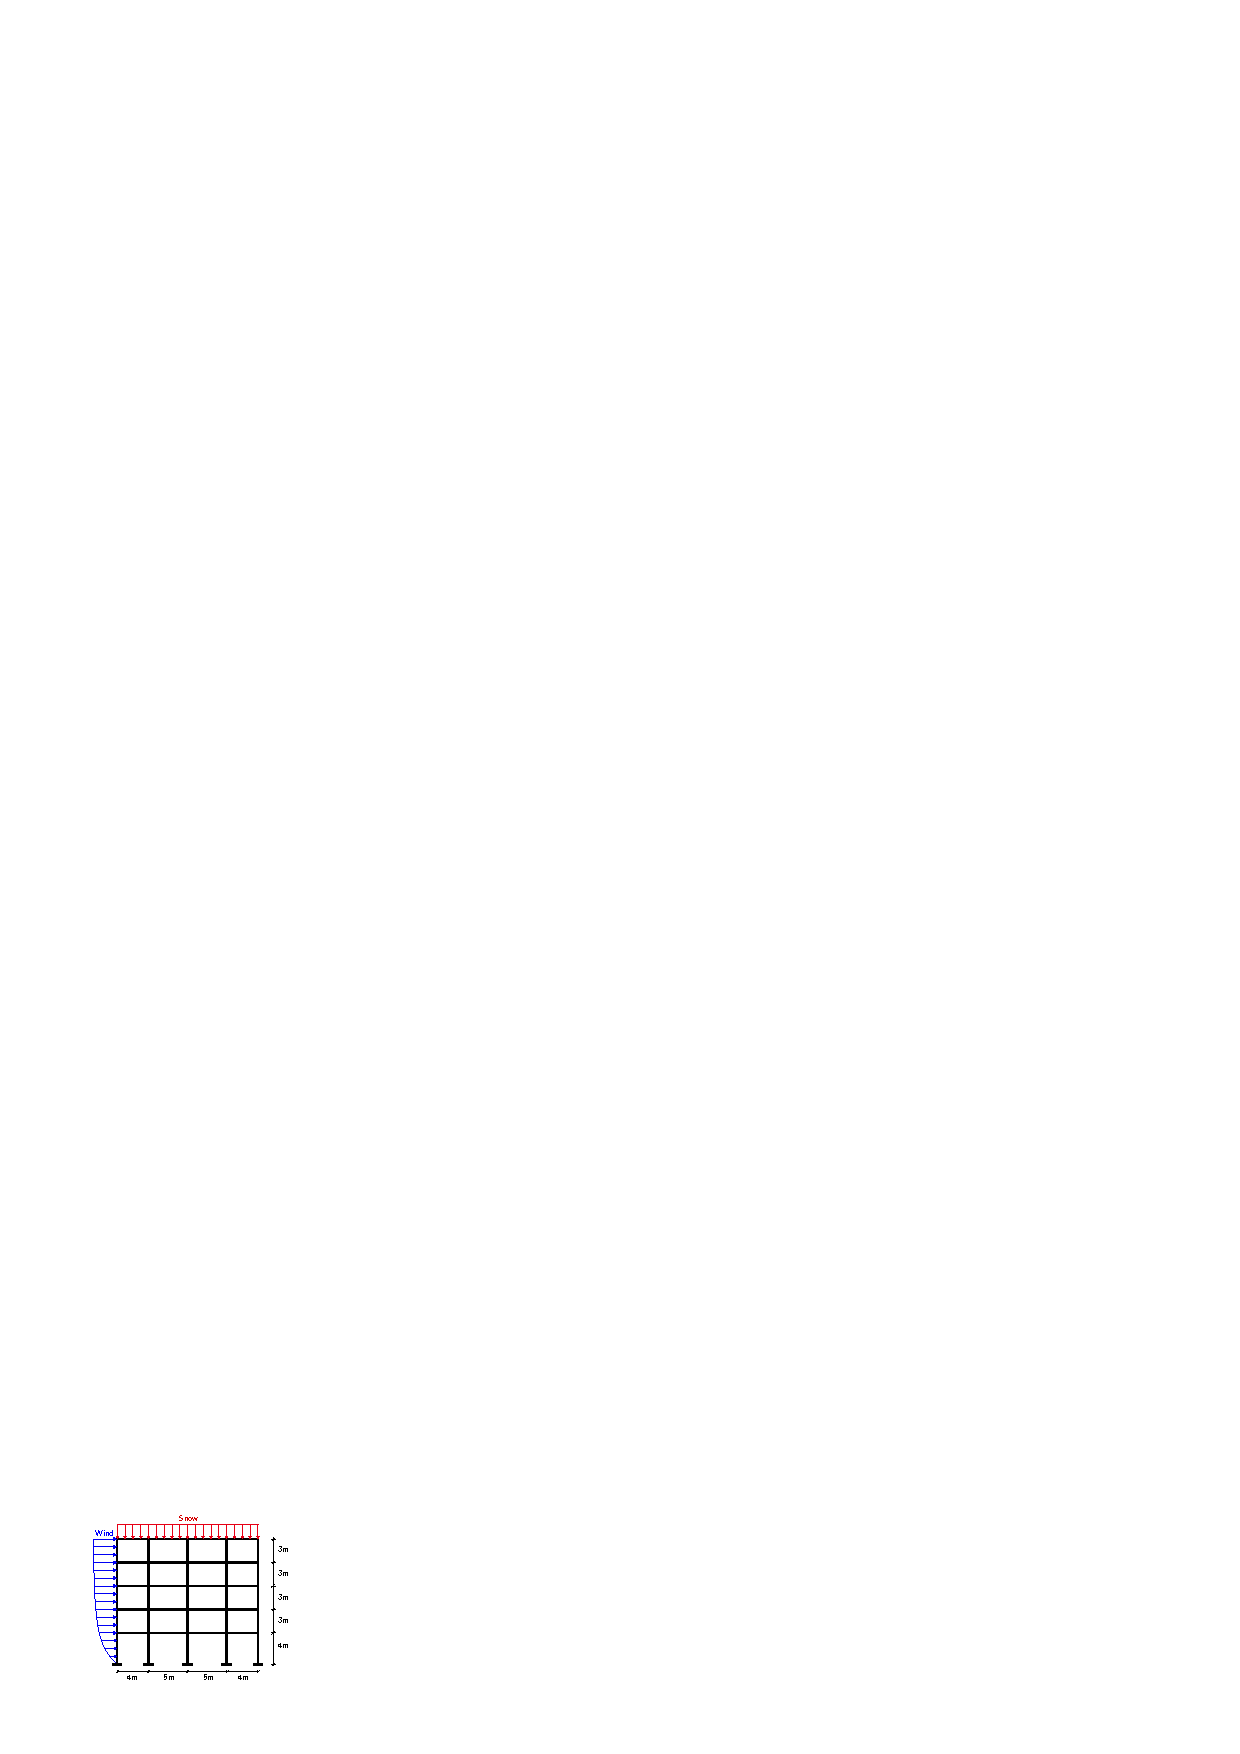
\includegraphics[width=0.7\textwidth]{RecorteP10}
\caption{Croquis de la edificación en 2D}
\label{fig:croquis}
\end{figure}


\end{document}

